%************************************************
\chapter{Sviluppo}\label{ch:sviluppo}
%************************************************
Il presente capitolo illustra come si è svolto il processo di sviluppo dei prototipi progettati, le problematiche riscontrate e le soluzioni che sono state applicate per risolverle.

La formazione iniziale sui framework da utilizzare è stata svolta su numerose e variegate fonti e con l'ausilio del tutor aziendale e di forum di supporto che hanno semplificato tale apprendimento e hanno contribuito a risolvere dubbi e difficoltà di vario genere.

Una lista esaustiva di tali fonti è da ricercarsi nella \hyperref[app:bibliography]{bibliografia}.

\section{MyNotes}
Lo sviluppo dell'applicazione \emph{MyNotes} ha richiesto uno studio approfondito del modulo \emph{SyncEngine}, tanto per comprenderne il funzionamento quanto per poterne implementarne le funzionalità all'interno dell'applicazione sviluppata.

\subsection{Studio SyncEngine}
Tale componente ha il compito di creare dinamicamente degli store da utilizzare per la gestione dei rispettivi modelli e di sincronizzare i dati inseriti dall'utente con un server predisposto.
Un punto critico di tale sistema è la potenziale distribuzione delle informazioni su più dispositivi; questo comporta l'unione dei dati in possesso di diversi utenti su di un unico database centralizzato in fase di upload e i possibili conflitti sui dati in fase di download a causa della presenza su di un device di dati locali non sincronizzati.

Il problema principale è stata la gestione degli ID dei record e le modifiche ai dati effettuabili da diversi utenti.
Il primo problema è stato parzialmente risolto con l'assegnamento di un codice identificativo ad ogni device, in modo da rendere unici i dati creati da ogni utente.
Il secondo ha richiesto la progettazione di un sistema ad hoc che utilizza store multipli per gestire l'unione dei record presenti nel database remoto con quelli locali in modo di garantire la consistenza globale dei dati.

Lo studio del \emph{SyncEngine} ha portato alla luce alcuni bug presenti in questo componente che non erano stati risolti dallo sviluppatore che ne ha curato la realizzazione:
\begin{itemize}
\item Il codice identificativo del device era cablato nel codice e, quindi, unico per tutte le installazioni dell'applicazione; si sono proposte due alternative:
	\begin{itemize}
	\item La creazione di una pagina dedicata alle informazioni del device in uso da compilare al primo avvio e dalla quale creare un ID univoco;
	\item L'utilizzo di un plugin di Apache Cordova che recupera l'\ac{UUID} proprio del dispositivo;
	\end{itemize}
\item Gli ID progressivi dei record inseriti vengono aggiunti dal sistema in modo automatico ma, ad ogni nuova installazione partono da $1$; in caso di reinstallazioni del software o di pulizia della cache insorgerebbero problemi di duplicazione di ID. Una soluzione potrebbe essere una richiesta al server per un controllo dell'esistenza dell'ID e l'ultimo codice progressivo utilizzato;
\item Ulteriori variabili cablate che facevano riferimento in modo stretto al prototipo realizzato per testare il componente; sono state modificate e rese parametriche per migliorare il riutilizzo del codice;
\item Nel \emph{SyncManager} erano assenti i metodi per effettuare la sincronizzazione con il server, si è quindi deciso di inserire i 2 metodi senza i quali tale funzionalità era nascosta allo sviluppatore:
	\begin{itemize}
	\item \code{downloadFromServer()};
	\item \code{uploadToServer()};
	\end{itemize}
\end{itemize}

\lstinputlisting[language=Java, caption={Metodi di sincronizzazione inseriti in \emph{SyncManager}}, label={lst:metodi sync manager}]{listings/metodi_sincro.java}

\subsection{Sviluppo interfaccia grafica}
Dopo aver compreso l'utilizzo del \emph{SyncEngine} si è iniziato lo sviluppo dell'applicazione seguendo la progettazione effettuata precedentemente.
Non conoscendo a priori le tecnologie utilizzate si è resa necessaria la consultazione di alcune guide online che trattassero gli argomenti richiesti: \emph{Sencha Touch 2.2.1}~\cite{sencha:touch221} con particolare attenzione al sistema delle classi, alla gestione automatica di getter e setter, al funzionamento generale del framework e all'utilizzo di \emph{Sencha Cmd} per creare lo scheletro dell'applicazione che si può vedere in figura \ref{fig:struttura app sencha touch}.

\begin{figure}[htb]
\centering
\includegraphics[scale=0.5]{gfx/screenshot/struttura_app}
\caption{Struttura file e cartelle applicazione Sencha Touch}
\label{fig:struttura app sencha touch}
\end{figure}

La cartella \emph{app} contiene i file sorgente del codice dell'applicativo divisi a seconda dei package, la cartella \emph{build} contiene i file prodotti dalla compilazione del sistema, la cartella \emph{packages} può contenere componenti di terze parti esterni all'applicazione come \emph{SyncEngine}, la cartella \emph{resources} contiene tutti i file che riguardano l'aspetto grafico, come immagini, fogli di stile, loghi e la cartella \emph{touch} contiene i file propri del framework utilizzato.

I file \emph{app.js} e \emph{index.html} sono i file principali dell'applicazione, il primo contiene la logica di inizializzazione mentre il secondo rappresenta la pagina principale della web app da cui viene caricato il file di inizializzazione.

Si è consultata inoltre una guida \cite{miamicoder:howto} che si è rivelata molto utile per comprendere il funzionamento del framework ed iniziare la stesura del codice.
Le maggiori difficoltà si sono incontrate nell'utilizzo dei componenti grafici da utilizzare per strutturare la \ac{GUI}: dalla documentazione di \emph{Sencha Touch} non è stato semplice capire come utilizzare tali componenti, in quanto spesso risulta essere frammentaria ed incompleta. Si è dovuto quindi procedere per gradi provando diverse soluzioni fino al raggiungimento del risultato desiderato.

\subsection{Integrazione SyncEngine}
Una volta realizzata l'interfaccia grafica è stato il momento di integrare il \emph{SyncEngine} nel prototipo: tale componente deve essere utilizzato come libreria esterna e, in questo caso, \emph{Sencha Touch} prevede l'utilizzo dei \emph{package}: questi sono dei moduli esterni che devono essere compilati in modo autonomo tramite un comando apposito e possono, in seguito, essere distribuiti senza rilasciare obbligatoriamente il codice sorgente.

Il modulo in questione non era stato preparato per tale scopo e si è quindi dovuto procedere ad effettuare la build di tale sistema: purtroppo è stato impossibile ottenere un prodotto utilizzabile nonostante i numerosi tentavi e la richiesta di aiuto al forum ufficiale Sencha \cite{sencha:buildingpackage}, dove inizialmente si è ricevuto supporto, ma, dopo alcuni scambi di messaggi, non si è giunti ad una soluzione.

Di fatto non è stato possibile integrare il \emph{SyncEngine} nel prototipo sviluppato utilizzando il sistema di build fornito da Sencha attraverso lo strumento \emph{Sencha Cmd}.

\subsection{Utilizzo Apache Cordova}
Giunti ad una situazione di stallo si è scelto di utilizzare Apache Cordova per completare la realizzazione di \emph{MyNotes}.

Dopo uno studio iniziale sul funzionamento del framework \cite{apache:cordova} e la lettura di diversi articoli pubblicati in internet \cite{andidog:packageSenchaPhonegap} \cite{sencha:senchaMVCphonegap} \cite{bgmemo:senchaPhonegap} per apprendere la tecnica per integrare il funzionamento di \emph{Sencha Touch} con \emph{Cordova}, si è riusciti nell'intento riuscendo ad ottenere un file \ac{APK} pronto per essere installato in qualsiasi device Android.
Il risultato è visibile in figura \ref{fig:screenshot mynotes}.

\begin{figure}[htb]
\centering
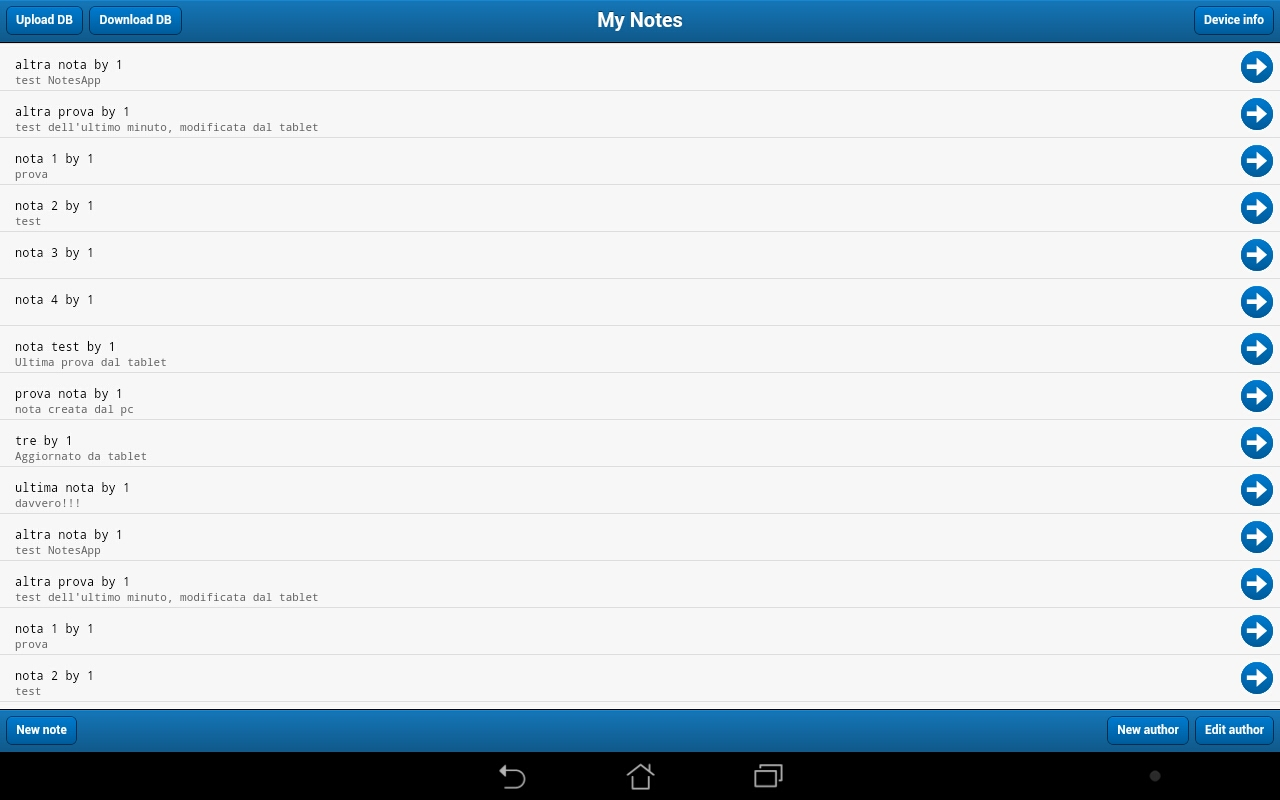
\includegraphics[scale=0.25]{gfx/screenshot/screen_MyNotes}
\caption{Screenshot pagina principale \emph{MyNotes}}
\label{fig:screenshot mynotes}
\end{figure}

\section{SensorDevice}
La realizzazione dell'applicazione \emph{SensorDevice} ha richiesto uno studio approfondito del framework \emph{Apache Cordova} \cite{apache:cordova} e del sistema di plugin che fornisce le interfacce alle funzionalità native dei device mobili.

Per soddisfare i requisiti dell'applicazione sono stati utilizzati i seguenti plugin:
\begin{description}
\item[Barcode\footnotemark:]\footnotetext{Plugin di terze parti \cite{wildabeast:barcodeScanner} trovato nella raccolta presente nel sito di \emph{PhoneGap}.} permette di leggere un barcode tramite la fotocamera del dispositivo;
\item[Camera:] permette di catturare un'immagine tramite la fotocamera o la galleria del dispositivo;
\item[Capture:] permette di catturare file audio, video e immagini tramite la fotocamera e il microfono del dispositivo ;
\item[Connection:] permette di testare la connettività del dispositivo e di recuperarne la tipologia;
\item[Contacts:] permette di consultare e modificare la rubrica del dispositivo;
\item[Device:] permette di visualizzare le informazioni proprie del dispositivo;
\item[File:] permette di scrivere o leggere un file nella memoria del dispositivo;
\item [Geolocation]: permette di visualizzare la posizione corrente del dispositivo;
\end{description}

\clearpage

\subsection{Sviluppo interfaccia grafica}

\begin{figure}[htb]
\centering
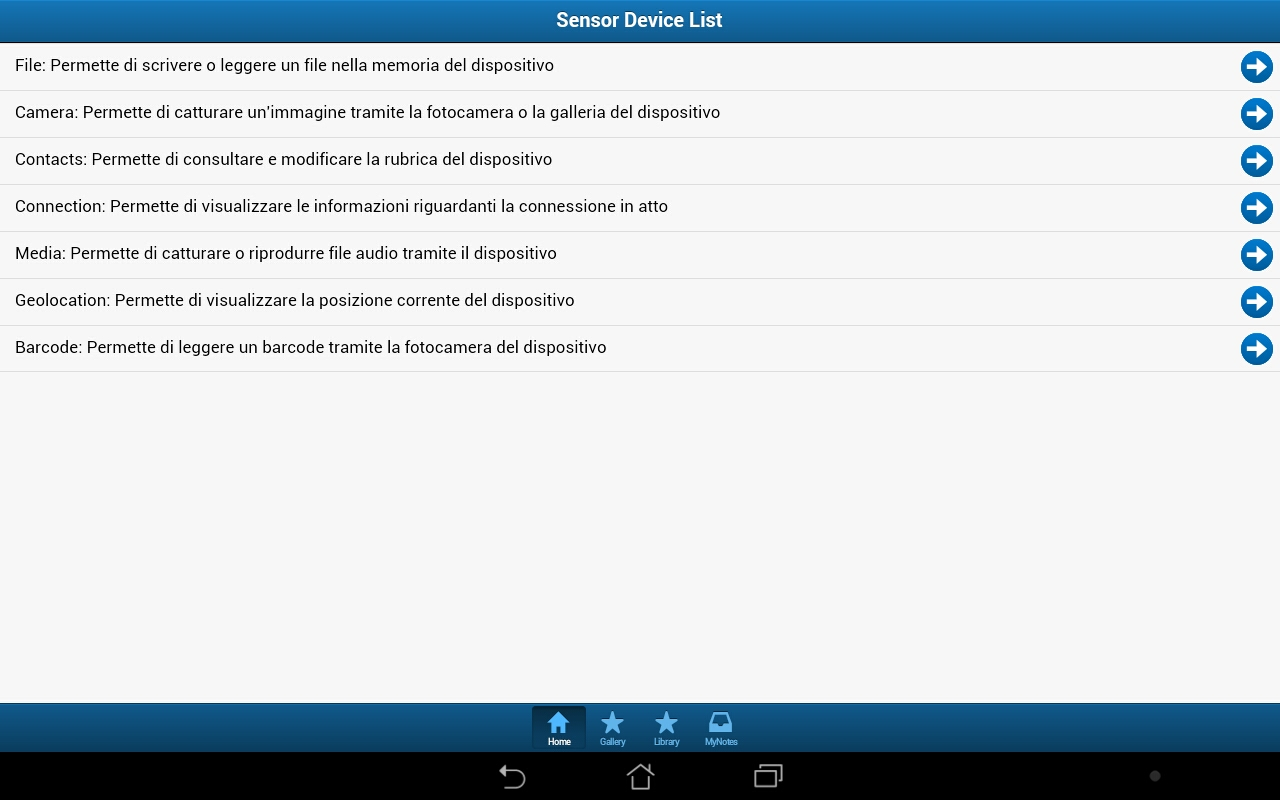
\includegraphics[scale=0.25]{gfx/screenshot/screen_sensorDevice}
\caption{Screenshot pagina principale \emph{SensorDevice}}
\label{fig:screenshot sensordevice}
\end{figure}

Lo sviluppo della \ac{GUI} ha prodotto il risultato visibile in figura \ref{fig:screenshot sensordevice}, dove si vede la lista di funzionalità utilizzabili dall'utente e in basso la barra di navigazione con le pagine disponibili.

L'interfaccia è volutamente molto semplice in quanto l'aspetto grafico non era tra gli obiettivi dello stage; la sua funzione, infatti, è solamente quella di illustrare all'utente le potenzialità offerte e permettergli di selezionarle.

La pagina che ha richiesto un lavoro più accurato è stata la form di compilazione delle informazioni personali dell'utente che viene utilizzata per realizzare il salvataggio dei dati nella memoria fisica del dispositivo; l'immagine è disponibile in figura \ref{fig:screenshot file sensordevice}.

\begin{figure}[htb]
\centering
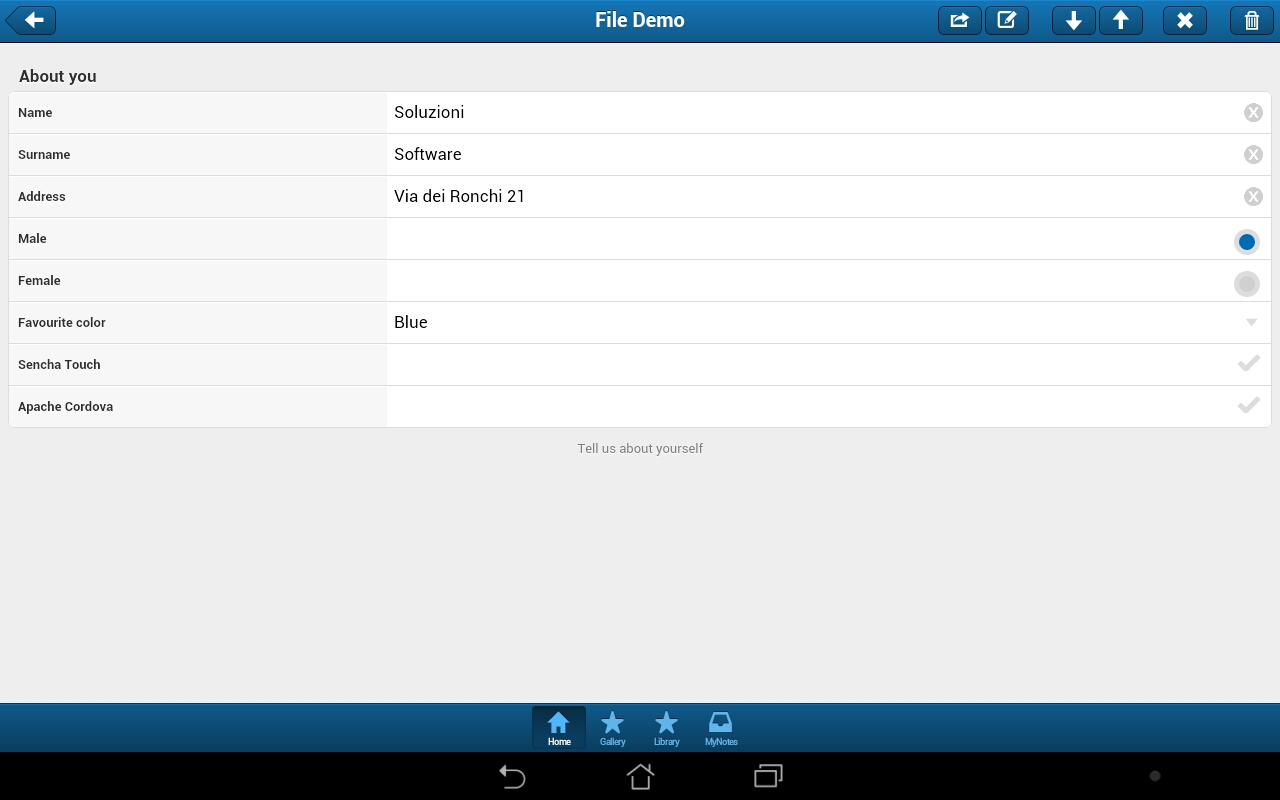
\includegraphics[scale=0.25]{gfx/screenshot/screen_file_sensorDevice}
\caption{Screenshot form informazioni personali \emph{SensorDevice}}
\label{fig:screenshot file sensordevice}
\end{figure}

\subsection{Utilizzo plugin Apache Cordova}
Il vantaggio nell'utilizzo di \emph{Cordova} risiede nella disponibilità di numerosi plugin che forniscono interfacce per le più comuni periferiche e funzionalità native dei device in commercio.

Grazie a tale caratteristica è stato semplice utilizzare le \ac{API} del framework per sviluppare i componenti previsti; la documentazione si è rivelata precisa ed affidabile e il tool a riga di comando ha completato con successo ogni tentativo di compilazione.

\subsection{Integrazione MyNotes}
L'ultimo passo per rendere completa l'applicazione è stato quello di integrare l'applicazione \emph{MyNotes} in una pagina di \emph{SensorDevice} in modo da fornire all'azienda una sola applicazione contenente tutto il lavoro svolto e che rendesse visibili tutte le funzionalità utilizzabili con l'utilizzo congiunto dei due framework utilizzati.

In figura \ref{fig:screenshot mynotes sensordevice} si può vedere la pagina relativa a \emph{MyNotes} all'interno di \emph{SensorDevice}; l'applicazione ha subito un naturale restyling dovuto alla diversa struttura grafica delle pagine ed è stata aggiunta la possibilità di salvare le note presenti sulla memoria del dispositivo.

\begin{figure}[htb]
\centering
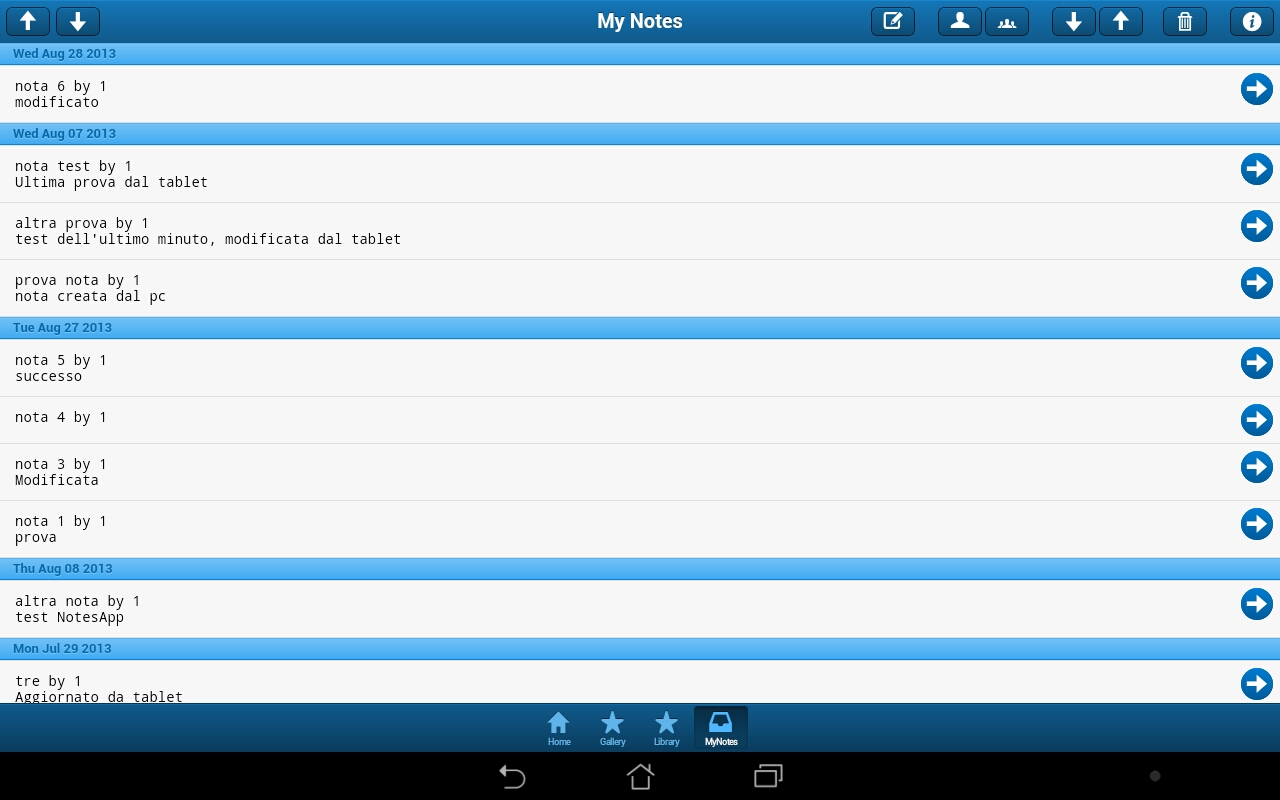
\includegraphics[scale=0.25]{gfx/screenshot/screen_sensor_myNotes}
\caption{Screenshot pagina \emph{MyNotes} integrata in \emph{SensorDevice}}
\label{fig:screenshot mynotes sensordevice}
\end{figure}

\section{ArchitectApp}
Con l'uscita di \emph{Sencha Touch 2.3} \cite{sencha:touch23} e dopo aver concluso positivamente i due prototipi, è stato effettuato uno studio sulle nuove caratteristiche offerte dal nuovo framework: in esso infatti sono stati aggiunte delle classi \emph{wrapper} alle \ac{API} di \emph{Cordova} rendendo ancora più semplice il lavoro dello sviluppatore.

Inoltre, è stato migliorato il tool di compilazione \emph{Sencha Cmd} che automaticamente richiama \emph{Cordova \ac{CLI}} per effettuare la build del sistema creando i file necessari per l'installazione sui dispositivi mobili.

Per provare questa nuova versione si è deciso di utilizzare \emph{Sencha Architect} \cite{sencha:architect}, strumento \emph{drag-and-drop} per la creazione di interfacce grafiche e di sfruttare l'incremento di velocità nello sviluppo per realizzare una nuova versione di \emph{SensorDevice}.

Si è iniziato a creare un'interfaccia ad hoc per tablet, divisa in due zone, una riservata al menu e l'altra studiata per ospitare i componenti utilizzati per visualizzare le funzionalità presenti all'utente.

Grazie a tale editor grafico è stato molto semplice creare una \ac{GUI} più complessa e articolata rispetto a quanto eseguito su editor testuale, evidenziando i pregi delle componenti grafiche del framework e sopperendo alle mancanze della documentazione spesso risulta essere molto enigmatica.

Il prodotto di questa attività è visibile in figura \ref{fig:screenshot device architect}, dove si può vedere la pagina che visualizza le informazioni proprie del dispositivo in uso ricavate con il relativo plugin di \emph{Apache Cordova}.

\begin{figure}[htb]
\centering
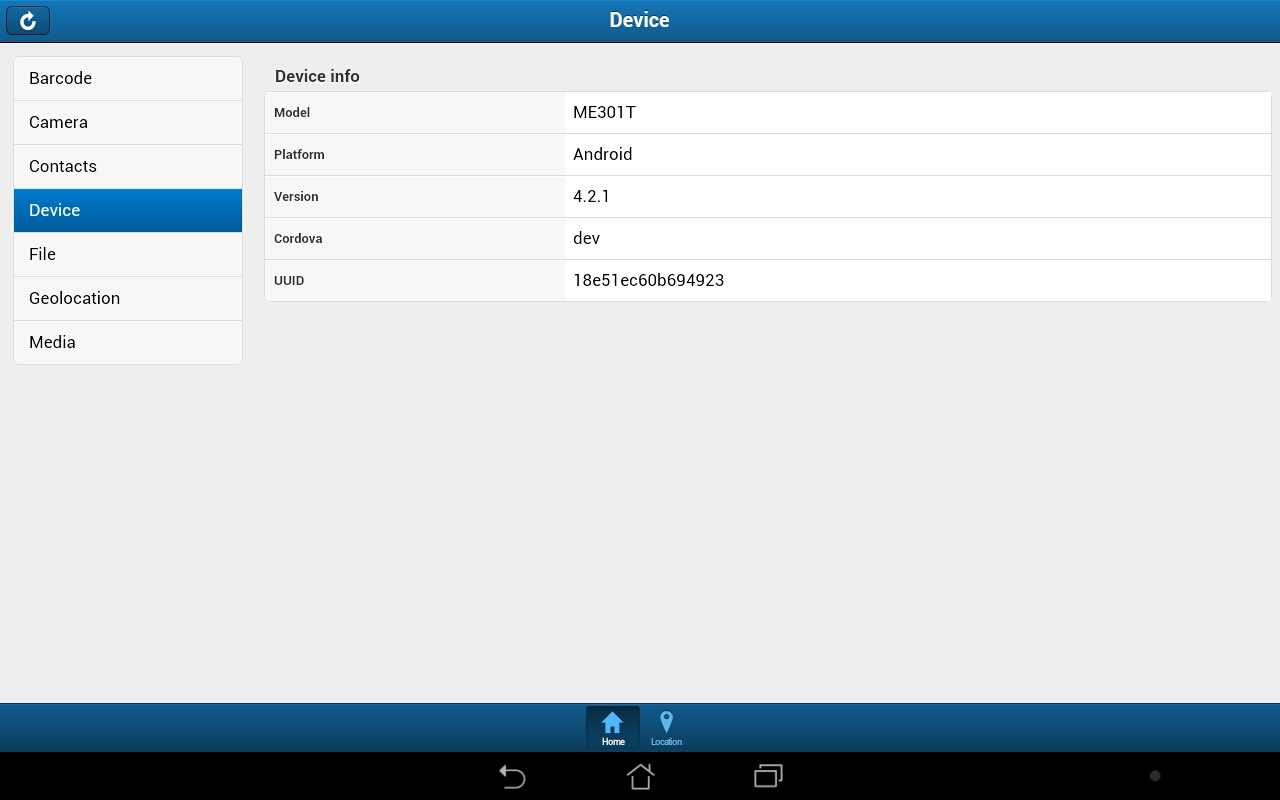
\includegraphics[scale=0.25]{gfx/screenshot/screen_device_architect}
\caption{Screenshot pagina informazioni device \emph{ArchitectApp}}
\label{fig:screenshot device architect}
\end{figure}